\tituloI{ASPECTOS ADMISNITRATIVOS}

\tituloII{Presupuesto}
\parrafoII{
El presupuesto del proyecto ha sido estructurado considerando los recursos necesarios para la ejecución del proceso experimental, incluyendo recursos humanos, infraestructura, servicios y costos operativos. Esta distribución permite garantizar la viabilidad técnica y económica del estudio.
}

\begin{table}[H]
\centering
\caption{Estructura del presupuesto ajustado del proyecto.}
\begin{tabular}{|l|l|c|c|c|c|}
\hline
\textbf{Categoría} & \textbf{Ítem} & \textbf{Cant.} & \textbf{Unidad} & \textbf{P. Unit (S/.)} & \textbf{Total (S/.)} \\ \hline

\multirow{2}{*}{Recursos Humanos}
& Investigador principal & 6 & mes & 0 & 0 \\ \cline{2-6}
& Asistente de investigación & 0 & mes & 0 & 0 \\ \hline

\multirow{2}{*}{Equipamiento}
& Estación de trabajo & 1 & unidad & 0 & 0 \\ \cline{2-6}
& Periféricos & 1 & lote & 200 & 200 \\ \hline

\multirow{2}{*}{Software}
& Herramientas open source & 1 & uso & 0 & 0 \\ \cline{2-6}
& Consumo API LLM & 1 & uso & 0 & 0 \\ \hline

\multirow{2}{*}{Servicios}
& Internet & 6 & mes & 100 & 600 \\ \cline{2-6}
& Electricidad & 6 & mes & 80 & 480 \\ \hline

\multirow{1}{*}{Otros}
& Impresión & 1 & lote & 150 & 150 \\ \hline

\multicolumn{5}{|r|}{\textbf{TOTAL}} & \textbf{1,430} \\ \hline
\end{tabular}
\end{table}
\parrafoII{
El experimento utilizará modelos de lenguaje de acceso gratuito o con planes académicos, lo cual elimina costos asociados al consumo de API, manteniendo la viabilidad económica del estudio. El proyecto será ejecutado por el investigador como parte de su formación académica, por lo que no se consideran costos salariales.
}

\parrafoII{
\textbf{Criterio de estimación:} El presupuesto prioriza el componente de recursos humanos, dado que la investigación se fundamenta en actividades de análisis, diseño experimental y validación. Los costos de software se mantienen reducidos debido al uso de herramientas open source, mientras que se considera un margen de contingencia para cubrir variaciones operativas.
}

\tituloII{Cronograma}
\parrafoII{
El cronograma del proyecto ha sido estructurado en un horizonte temporal de 24 semanas, comprendido entre julio y diciembre de 2026. Se ha definido una secuencia lógica que integra actividades de investigación, desarrollo experimental y validación, permitiendo la superposición controlada de tareas para optimizar el tiempo de ejecución.
}

\begin{figure}[H]
\centering
\caption{Cronograma del proyecto elaborado en ProjectLibre}
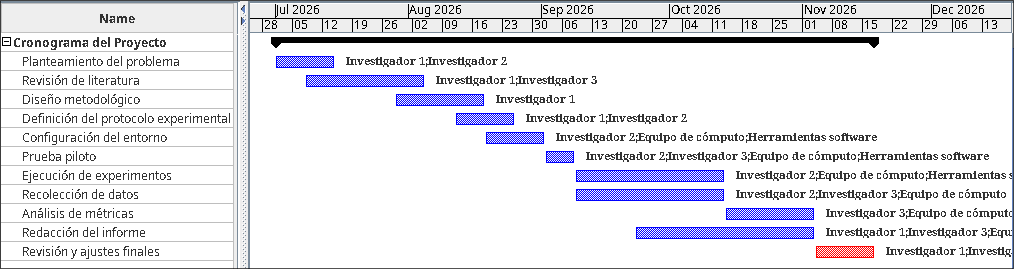
\includegraphics[width=0.95\textwidth]{gantt.png}
\label{fig:gantt}
\end{figure}

\parrafoII{
\textbf{Criterio de planificación:} Se ha optado por un enfoque semi-paralelo en la ejecución de actividades críticas, particularmente en la fase experimental, donde la generación de código y la recolección de datos se desarrollan de manera concurrente. Esta estrategia reduce el tiempo total del proyecto sin comprometer la validez de los resultados.
}
